\section*{Results}

\subsection*{Constant function}

\begin{center}
    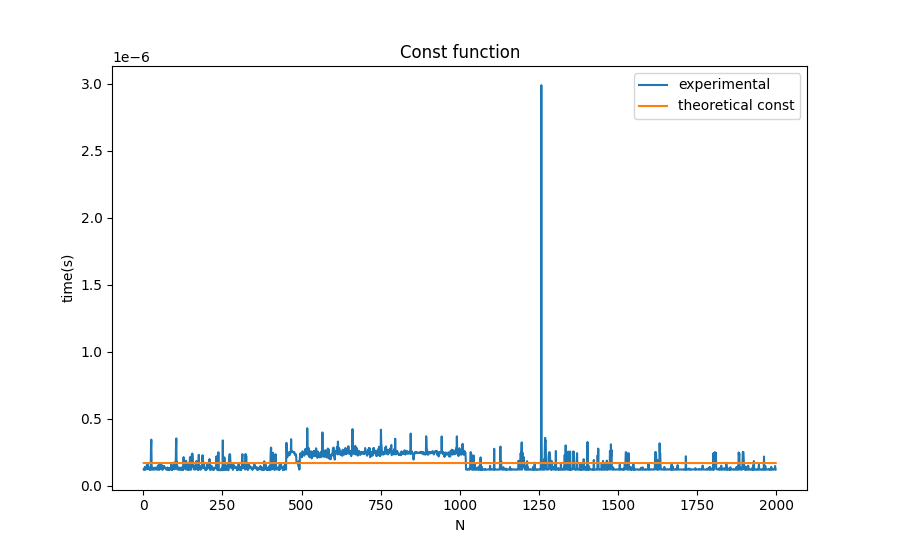
\includegraphics[width=0.6\textwidth]{../results/const_f.png}
    \captionof{figure}{Execution time of constant function}
\end{center}

As it can be seen execution time does not depends on number of elements in array. Altough there some noise in experimental data.

\subsection*{Sum function}

\begin{center}
    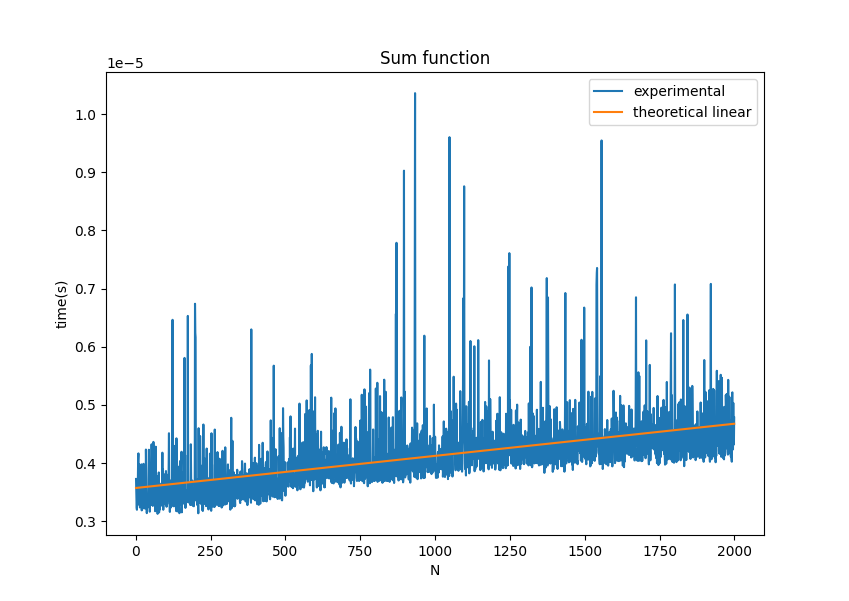
\includegraphics[width=0.6\textwidth]{../results/sum_f.png}
    \captionof{figure}{Execution time of sum function}
\end{center}

\subsection*{Product function}

\begin{center}
    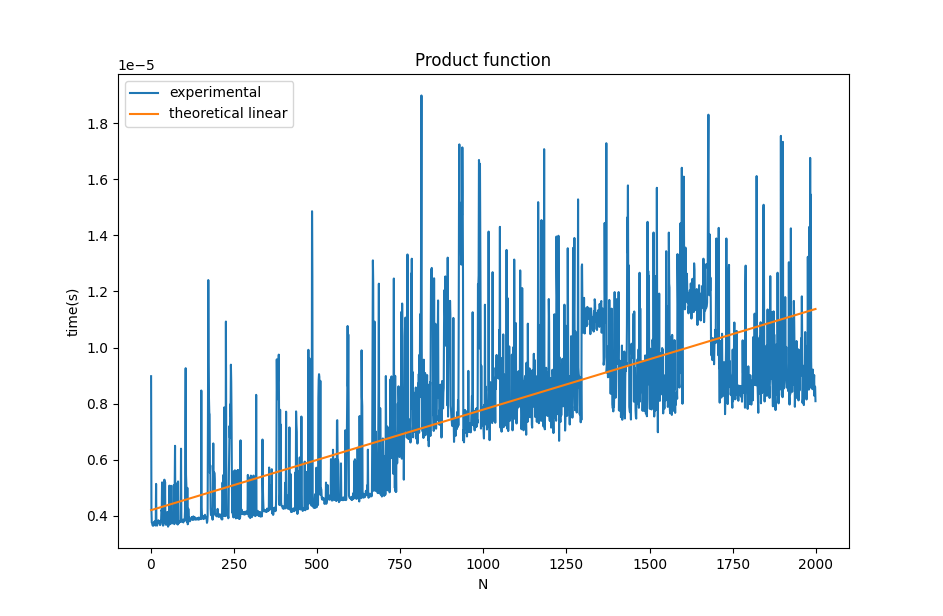
\includegraphics[width=0.6\textwidth]{../results/product_f.png}
    \captionof{figure}{Execution time of product function}
\end{center}

For both sum and product function the experimental data can be closely described by linear functions.

\subsection*{Polynomial}

\begin{center}
    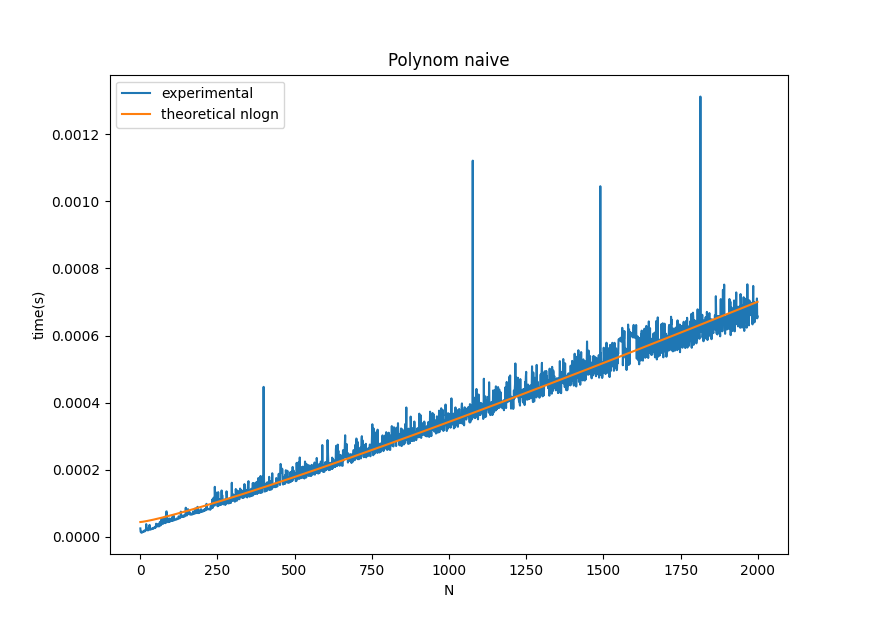
\includegraphics[width=0.6\textwidth]{../results/polynom_naive.png}
    \captionof{figure}{Execution time of naive polynomial function}
\end{center}

\begin{center}
    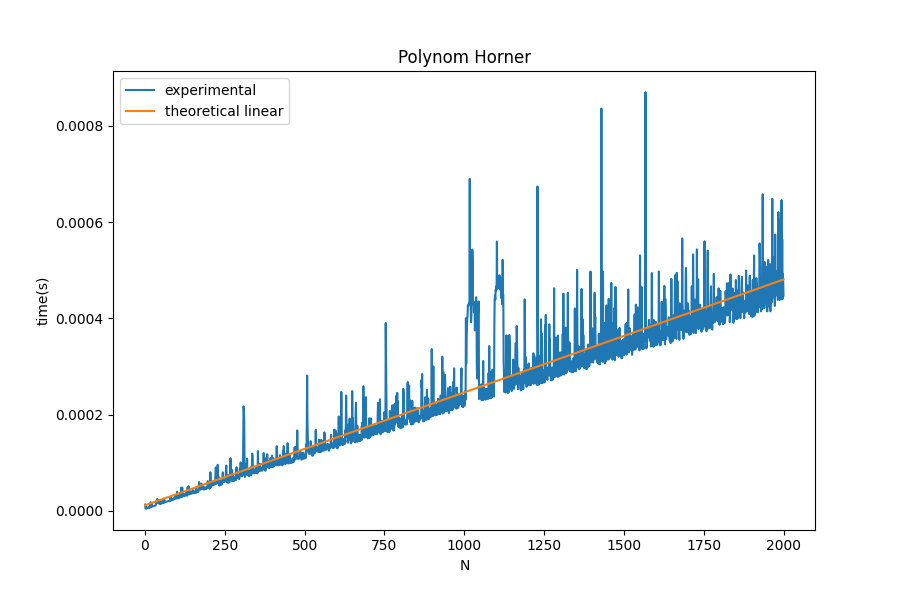
\includegraphics[width=0.6\textwidth]{../results/polynom_horner.png}
    \captionof{figure}{Execution time of Horner's polynomial function}
\end{center}

As it can be seen Horner's method execution time can be described by linear function, moreover naive polynomial can be described
closely with linear function on that subset of input data. That can be explained by lower constant of $NlogN$ term of time complexity. However, already on such small data sizes (2000) optimized version shows slightly better results.

\subsection*{Sorts}

\begin{center}
    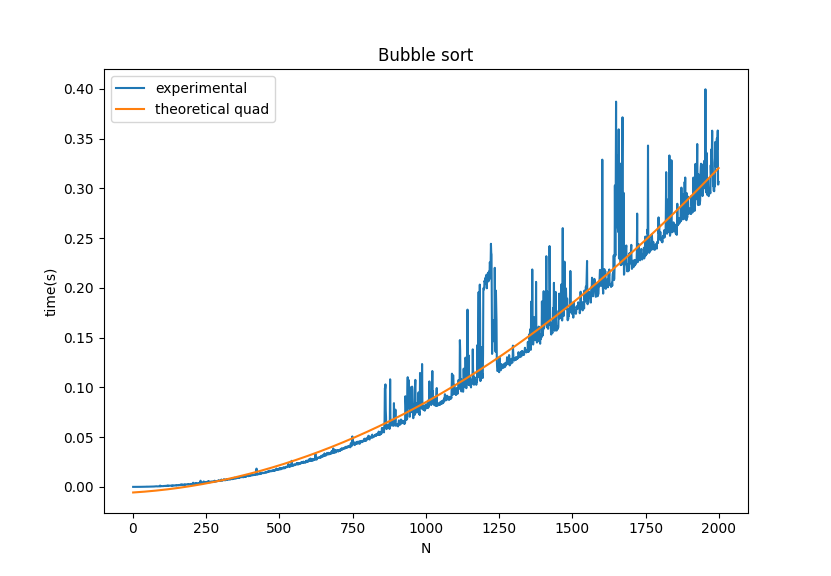
\includegraphics[width=0.6\textwidth]{../results/bubble_sort.png}
    \captionof{figure}{Execution time of Bubble sort}
\end{center}

\begin{center}
    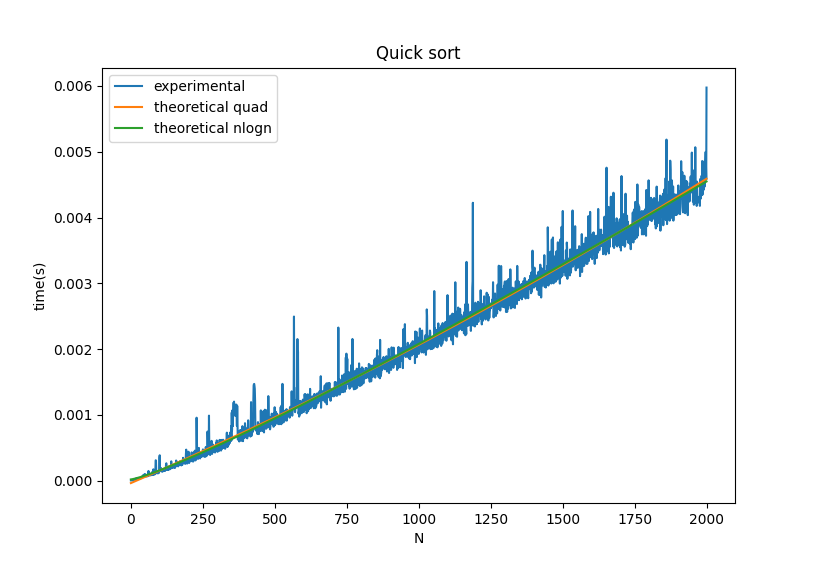
\includegraphics[width=0.6\textwidth]{../results/quick_sort.png}
    \captionof{figure}{Execution time of Quicksort}
\end{center}

In that figure can execution time of quicksort can be better described with $NlogN + C$ function or $a n^2 + b n + c$ (that describes worst case of quicksort) with low $a$ value (that is closer to linear function).
That caused by the fact that measurements were taken on random vectors and shows the average execution time of function. 

\begin{center}
    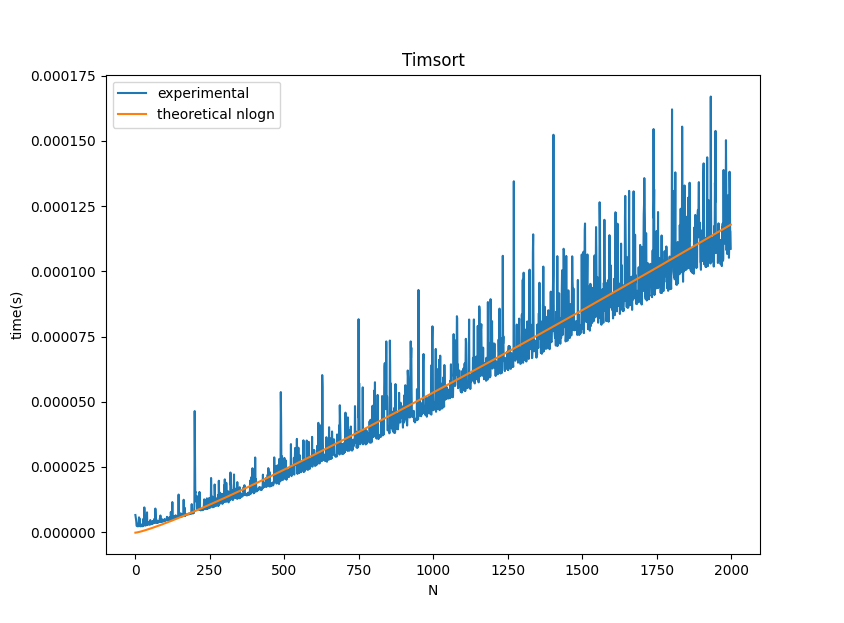
\includegraphics[width=0.6\textwidth]{../results/timsort.png}
    \captionof{figure}{Execution time of Timsort}
\end{center}

\subsection*{Matrices product}

\begin{center}
    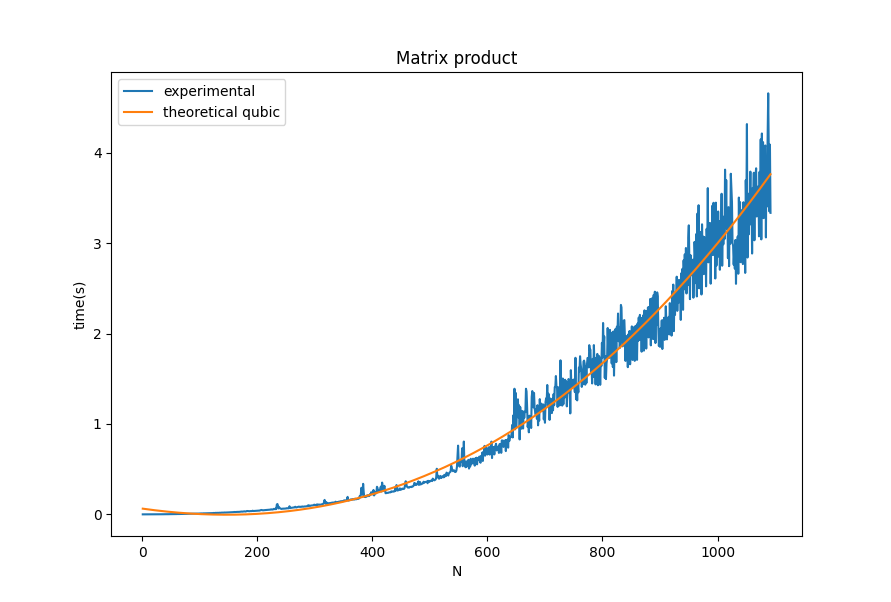
\includegraphics[width=0.6\textwidth]{../results/matrix_product.png}
    \captionof{figure}{Execution time of matrices product}
\end{center}